\documentclass[12pt]{article}

\usepackage[utf8]{inputenc}
\usepackage[T1]{fontenc}
\usepackage{amsmath}
\usepackage{amssymb}
\usepackage{graphicx}
\usepackage{booktabs}
\usepackage{hyperref}
\usepackage[round]{natbib}
\usepackage{tikz}
\usetikzlibrary{arrows.meta, positioning, calc, backgrounds, fit, decorations.pathreplacing}
\usepackage[margin=1in]{geometry}

\title{Designing Institutional Forgetting for AI Agent Memory Systems}
\author{Jiyeon Yoon\\
Independent Researcher\\
\texttt{heznpc@gmail.com}}
\date{}

\begin{document}

\maketitle

\begin{abstract}
AI memory systems treat forgetting as deletion. Time-to-live policies erase records after a fixed interval; machine unlearning attempts to excise data from model weights; GDPR erasure requests demand that information be removed on command. Yet the oldest human institution designed for forgetting---the statute of limitations, first documented in fifth-century BCE Athens---does none of these things. It does not delete evidence, silence witnesses, or erase the historical record. It extinguishes the authority to act on information, not the information itself. The Hwaseong serial murder case in South Korea illustrates the distinction with painful clarity: when DNA evidence identified the killer in 2019, the investigative files were intact, the confession was forthcoming, but prosecution was impossible---the data existed, yet the authority to act on it had expired. This paper traces 2,500 years of institutional forgetting across six civilizational traditions---Athenian, Roman, Confucian, Islamic, Germanic, and common law---and extracts seven design principles for AI agent memory governance. We propose the \emph{sihyo} architecture, a three-layer framework in which information persists indefinitely in a memory store, an authority registry tracks expiration status for each memory, and a decision layer consults the registry before acting. Unlike existing approaches that equate forgetting with deletion, sihyo separates storage from authority, enabling severity-proportional expiration, suspension conditions, reactivation mechanisms, and non-retroactive policy changes. We situate the framework against current systems including Mem0, MemOS, and Governed Memory, identify three boundary conditions where the model fails, and argue that the equation ``forgetting equals deletion'' represents not a technical constraint but a design poverty that 2,500 years of legal history has already resolved.
\end{abstract}

% ============================================================================
\section{Introduction}
\label{sec:introduction}
% ============================================================================

On September 18, 2019, South Korean police announced that DNA analysis had identified Lee Chun-jae as the perpetrator of the Hwaseong serial murders---a string of ten rape-murders committed between 1986 and 1991 that had haunted the nation for three decades. The evidence was unambiguous: DNA recovered from victims' clothing matched Lee's profile across multiple cases. Lee himself confessed, eventually admitting to fourteen murders and thirty sexual assaults. The investigative files were intact. The witnesses were available. The forensic evidence was conclusive.

None of it mattered. The statute of limitations for each murder had expired between 2001 and 2006, fifteen years after each crime. Lee could not be prosecuted for the Hwaseong killings. The information existed in full; the authority to act on it had been extinguished by time.

The Hwaseong case is not merely a legal curiosity. It is a precise illustration of a design paradigm that the artificial intelligence community has almost entirely overlooked. When AI researchers and system designers talk about ``forgetting,'' they mean deletion: time-to-live (TTL) policies that erase database entries, machine unlearning algorithms that attempt to remove information from model weights, GDPR erasure requests that demand data be destroyed on command. In every case, the operative assumption is the same: to forget is to delete, and to delete is to render information as if it never existed.

The statute of limitations operates on a fundamentally different logic. It does not delete evidence from police archives. It does not erase memories from witnesses' minds. It does not destroy the historical record. What it does---and what it has done across every civilization that has adopted it over the past 2,500 years---is sever the connection between information and action. The data persists; the authority to act on it expires.

This paper argues that the conflation of forgetting with deletion is not a technical constraint but a design poverty, and that the statute of limitations offers a richer, more nuanced paradigm for AI agent memory governance. We trace the history of institutional forgetting across six civilizational traditions, extract seven design principles from this cross-cultural record, and propose the \emph{sihyo} architecture---a three-layer framework in which information persists indefinitely while the authority to act on it expires according to configurable, severity-proportional rules.

% ----------------------------------------------------------------------------
\subsection{The Fundamental Asymmetry}
\label{sec:fundamental-asymmetry}
% ----------------------------------------------------------------------------

The need for such a framework arises from a fundamental asymmetry between human and digital memory. Human memory forgets by default: remembering requires effort, attention, and rehearsal, while forgetting occurs naturally through interference, decay, and consolidation \citep{ricoeur-memory}. Digital memory preserves by default: every interaction is logged, every token stored, every embedding persisted, while deletion requires explicit action---engineering resources, policy decisions, and regulatory compliance.

The statute of limitations was, in its original context, a solution to precisely this kind of asymmetry. Ancient societies did not face the problem of perfect digital recall, but they did face a version of the same challenge: once a legal claim was recorded and a prosecution initiated, the machinery of the state could pursue it indefinitely. The accuser could hold the threat of litigation over the accused for years or decades. Evidence might decay, but the institutional memory of the claim did not. Athens, Rome, and every subsequent legal tradition that adopted statutes of limitations were, in effect, designing institutional forgetting for systems that did not forget on their own.

AI agent memory systems face the same structural problem in a more extreme form. A long-running agent accumulates memories---user preferences, factual corrections, safety incidents, conversational context---and these memories persist indefinitely unless explicitly managed. Over time, outdated preferences override current ones, obsolete facts contaminate reasoning, and the sheer volume of accumulated context degrades performance. The system remembers everything and forgets nothing, not because remembering is valuable but because deletion was never designed into the architecture.

What these systems lack is not a deletion mechanism---TTL policies are trivial to implement---but a \emph{forgetting} mechanism in the richer sense that human institutions have developed over millennia: one that manages the relationship between information and action without destroying the information itself. The statute of limitations is the oldest, most thoroughly tested, and most cross-culturally validated instance of such a mechanism. This paper extracts its design principles and proposes their application to AI agent memory governance.

% ============================================================================
\section{Background: How Societies Designed Forgetting}
\label{sec:background}
% ============================================================================

% ----------------------------------------------------------------------------
\subsection{Origins and Evolution}
\label{sec:origins}
% ----------------------------------------------------------------------------

The earliest documented statute of limitations appears in fifth-century BCE Athens, where a five-year limitation period (\emph{prothesmia}) applied to nearly all offenses except murder \citep{demosthenes}. The Athenian institution is notable less for its specific time limits than for its explicit justification: Demosthenes records that the \emph{prothesmia} was designed to control \emph{sycophants}---professional accusers who exploited the legal system by threatening prosecution for personal gain. The statute of limitations was, from its inception, a mechanism for preventing system abuse, not an expression of mercy toward offenders.

Roman law developed the concept along a parallel but distinct trajectory. The Twelve Tables (c.~450 BCE) introduced \emph{usucapio}, a form of acquisitive prescription under which continuous possession of movable property for one year, or immovable property for two years, conferred ownership. This was not a limitation on prosecution but a rule by which the passage of time created new legal facts---a principle that would prove foundational. The praetorian system later imposed one-year limits (\emph{annus utilis}) on newly created actions, and Augustus's \emph{Lex Julia de Adulteriis} (18 BCE) established sixty-day and six-month prosecution windows for adultery.

The decisive Roman innovation came in 424 CE, when Theodosius II imposed a thirty-year limitation period (\emph{praescriptio triginta annorum}) on all previously perpetual actions \citep{codex-theodosianus}. This was, for the first time, a systematic assertion that no legal claim should persist indefinitely---that the state's authority to act must have a temporal boundary. Justinian's sixth-century codification unified acquisitive and extinctive prescription into a coherent framework, establishing the conceptual vocabulary that would shape Continental European law for the next fifteen centuries.

The justification logic for these institutions evolved over time in a pattern that is itself instructive for AI system design. Athens justified limitation periods as abuse prevention---a system-level concern. Rome shifted toward legal stability and administrative efficiency---state-level concerns. Medieval canon law added theological dimensions, framing prescription as necessary for social peace and the repose of the soul. Early modern Continental law emphasized evidence decay---an epistemological concern about the reliability of information over time. Modern criminal law grounds limitation periods in the human rights of the accused---the right not to live under indefinite threat of prosecution. Each era added a new justification without entirely discarding the old ones, producing a layered rationale that reflects the genuine complexity of the problem.

% ----------------------------------------------------------------------------
\subsection{Cross-Cultural Taxonomy of Forgetting Design}
\label{sec:taxonomy}
% ----------------------------------------------------------------------------

The statute of limitations is not a single design but a family of designs. Different civilizations, confronting the same fundamental tension between remembering and acting, arrived at markedly different solutions. Table~\ref{tab:taxonomy} presents a taxonomy of six design models, each with a distinct logic and a corresponding analogy to AI memory architecture.

\begin{table}[ht]
\centering
\caption{Cross-cultural taxonomy of forgetting design.}
\label{tab:taxonomy}
\begin{tabular}{@{}lll@{}}
\toprule
Design Model & Civilizations & AI Memory Analogy \\
\midrule
No forgetting (perpetual) & Confucian East Asia & Unlimited context, no eviction \\
Dual-rights hierarchy & Islamic law & System safety (no TTL) vs.\ user prefs (TTL) \\
Codified uniform decay & Roman / Continental & Uniform TTL for all memory types \\
Pragmatic incremental & English common law & Ad hoc retention policies \\
Severity-proportional & Modern criminal law & Memory-type-proportional TTL \\
Abolition after failure & Korea, Japan, Germany & Policy reversal after visible harm \\
\bottomrule
\end{tabular}
\end{table}

The perpetual-memory model, characteristic of Confucian legal traditions in China, Korea, and Japan before Western legal influence, treated all offenses as moral violations that could not expire with time. The dual-rights hierarchy of Islamic jurisprudence distinguished between claims belonging to God (\emph{huquq Allah}), which could not expire, and claims belonging to individuals (\emph{huquq al-ibad}), which could. Roman and Continental European law imposed uniform limitation periods---Theodosius's thirty years, eventually shortened to three years in Germany's 2002 reform---that applied regardless of offense severity. English common law developed limitation periods piecemeal, producing the Limitation Act of 1623 \citep{limitation-act-1623} with its six-year default whose rationale the English Law Commission later admitted it could not reconstruct. Modern criminal law systems graduated limitation periods by offense severity, from one to three years for misdemeanors to perpetual prosecution authority for murder. And the abolition cases---Germany, Japan, Korea---represent moments when societies reversed their forgetting policies after catastrophic failures made the costs of forgetting visible.

Each of these models encodes a different answer to the question that every AI memory system must also confront: what should happen to information over time? The taxonomy demonstrates that this question has no single correct answer, but it has a rich space of well-tested solutions.

% ----------------------------------------------------------------------------
\subsection{The Abolition Cases: What Happens When Forgetting Fails}
\label{sec:abolition-cases}
% ----------------------------------------------------------------------------

Three cases of statute-of-limitations abolition in the twentieth and twenty-first centuries reveal a consistent pattern that is directly relevant to AI memory governance: societies abolish forgetting policies when new technology or new circumstances invalidate the original justification for those policies.

\textbf{Germany, 1965--1979.} The West German criminal code set a twenty-year statute of limitations for murder. As this deadline approached for Nazi-era war crimes in the 1960s, a fierce parliamentary debate erupted. The Bundestag extended the limitation period twice---first to 1969, then to 1979---before abolishing it entirely for murder in a dramatic televised vote on July 3, 1979 (255 to 222) \citep{german-verjaehrung}. The core argument for abolition was that the original justification for limitation periods---evidence decay, diminished social interest in punishment, rehabilitation of the offender---did not apply to genocide and crimes against humanity. The severity of the offense overwhelmed the institutional logic of forgetting.

\textbf{Japan, 2010.} Japan's criminal procedure code, modeled on German law, set a fifteen-year statute of limitations for capital offenses. In 2004, this was extended to twenty-five years. On April 27, 2010, the Diet abolished the statute of limitations for all crimes punishable by death. Minister of Justice Keiko Chiba ordered immediate enforcement on the same day---because a 1995 unsolved murder case was set to expire at midnight. The amended law applied retroactively to all cases whose statutes had not yet expired, saving an unknown number of open investigations from automatic closure.

\textbf{Korea, 2015.} South Korea's statute of limitations for murder was originally fifteen years, extended to twenty-five in 2007. Between January and April 2006, several high-profile cases expired in rapid succession, including one of the Hwaseong serial murder cases. The case of a six-year-old boy named Taewan, killed in a sulfuric acid attack whose perpetrator could not be prosecuted before the statute expired, catalyzed public outrage. In July 2015, the National Assembly passed the Taewan Act, abolishing the statute of limitations for first-degree murder \citep{korea-taewan}. Critically, the law was \emph{not} retroactive: cases whose statutes had already expired remained closed. When DNA identified Lee Chun-jae as the Hwaseong killer four years later, the investigative files were intact but the authority to prosecute had already been extinguished.

The common pattern across these three cases is instructive. In each instance, abolition was triggered by the convergence of two factors: (1) new technology---primarily DNA forensics---that undermined the evidence-decay justification for limitation periods, and (2) a specific, emotionally salient case that made the costs of the existing policy visible to the public. The technology changed what was \emph{possible}; the case changed what was \emph{tolerable}. For AI memory governance, this pattern suggests that forgetting policies will inevitably require revision as capabilities evolve, and that the design of such policies should anticipate the need for principled, non-disruptive updating.

% ============================================================================
\section{The Missing Paradigm: Exists But Doesn't Act}
\label{sec:missing-paradigm}
% ============================================================================

% ----------------------------------------------------------------------------
\subsection{Current AI Memory Forgetting Models}
\label{sec:current-models}
% ----------------------------------------------------------------------------

The growing literature on AI agent memory has begun to address the problem of memory management, but every proposed solution to date operates within the deletion paradigm. Table~\ref{tab:current-models} summarizes the five principal approaches and their limitations.

\begin{table}[ht]
\centering
\caption{Current AI memory forgetting approaches and their limitations.}
\label{tab:current-models}
\begin{tabular}{@{}lll@{}}
\toprule
Approach & Mechanism & Problem \\
\midrule
TTL / Expiration & Delete after time & Information irrecoverably lost \\
Machine unlearning & Remove from weights & Technically fails \citep{unlearning-iclr2025} \\
GDPR erasure & Delete on request & Reactive, not systematic \\
Temporal decay & Reduce retrieval weight & Uniform, no severity distinction \\
Context window truncation & Drop oldest tokens & Accidental, not designed \\
\bottomrule
\end{tabular}
\end{table}

\emph{TTL-based expiration} is the most common approach in production systems. Mem0 \citep{mem0-2025} and similar memory layers allow developers to set time-to-live values for stored memories, after which the entries are deleted. The mechanism is simple and predictable, but it destroys information irrecoverably. A user preference that was valid six months ago and might become valid again is indistinguishable from one that was always wrong---both are gone.

\emph{Machine unlearning} attempts to remove specific data points from trained model weights, offering the promise of targeted forgetting without full retraining. However, recent work has demonstrated that current unlearning techniques fail to fully remove the influence of targeted data \citep{unlearning-iclr2025}. The fundamental obstacles are verification (there is no reliable way to confirm that unlearning has occurred), utility degradation (aggressive removal damages performance on unrelated tasks), and scale (techniques validated on small classifiers do not extend to models with billions of parameters).

\emph{GDPR-style erasure} responds to explicit user requests by deleting personal data from storage. This approach is reactive rather than systematic---it requires the data subject to identify what should be forgotten and to initiate the request. It provides no mechanism for the system to manage its own memory proactively.

\emph{Temporal decay} reduces retrieval weights for older memories, making them less likely to influence current behavior without deleting them outright. This is the approach closest to the statute-of-limitations paradigm, but existing implementations apply uniform decay regardless of memory type or severity. A safety-critical lesson from a dangerous interaction decays at the same rate as a formatting preference, which is analogous to a legal system that applies the same limitation period to jaywalking and murder.

\emph{Context window truncation} is not a designed forgetting mechanism at all but an accidental one: when an agent's context exceeds its window limit, the oldest tokens are dropped. This is the digital equivalent of a filing cabinet that, when full, discards whatever is at the bottom of the pile. It is not forgetting by design but forgetting by overflow.

MemOS \citep{memos-2025} proposes an operating-system metaphor for agent memory, managing storage, retrieval, and scheduling across heterogeneous memory types. Governed Memory \citep{governed-memory-2026} introduces policy-based memory governance with access controls and retention rules. The broader survey by \citet{memory-ai-agents-2025} maps the landscape of memory architectures for AI agents. None of these systems, however, implements the core distinction that the statute of limitations embodies: the separation of information persistence from action authority.

Figure~\ref{fig:memory-governance-comparison} illustrates this distinction. The left panel shows the deletion paradigm shared by all current approaches: data is stored, time elapses, and the data is destroyed with no possibility of recovery. The right panel shows the authority-expiration paradigm that the statute of limitations embodies: data persists indefinitely, but its authority to influence decisions expires---and can be restored when new context warrants it.

\begin{figure}[htbp]
\centering
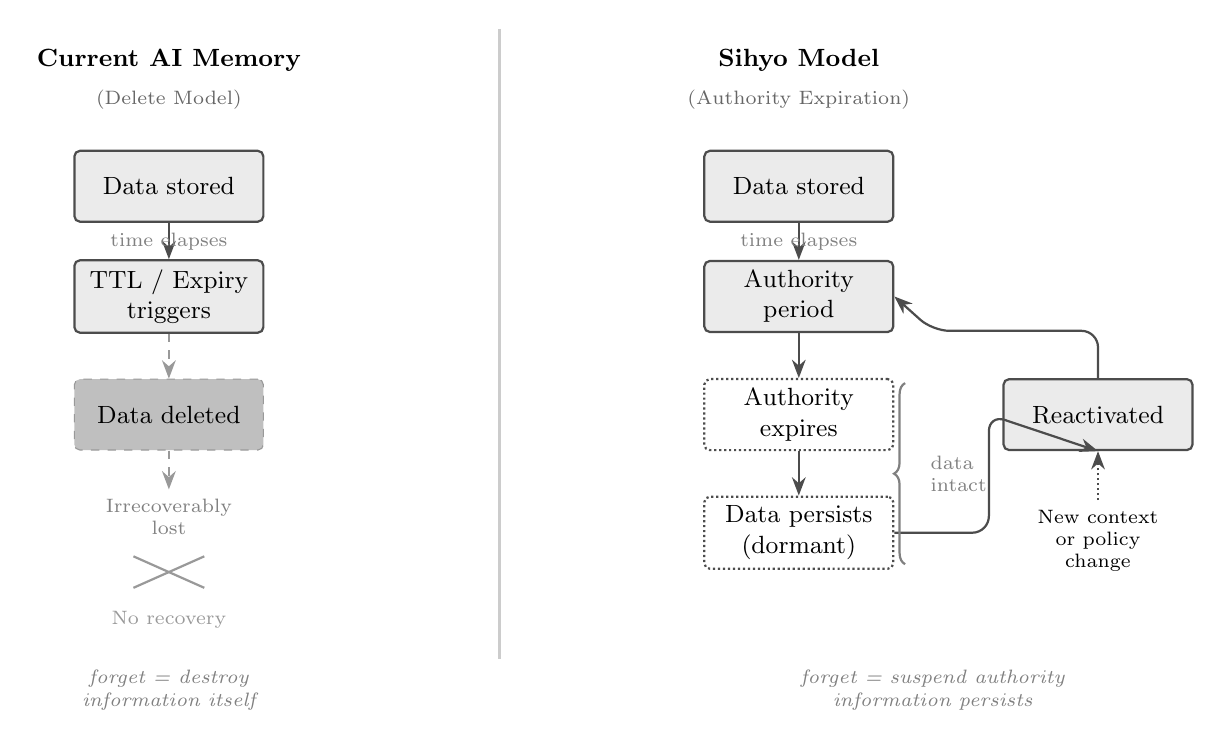
\begin{tikzpicture}[
    >=Stealth,
    node distance=0.7cm and 0.5cm,
    box/.style={rectangle, draw, rounded corners=2pt, minimum height=0.9cm,
                minimum width=2.4cm, align=center, font=\small},
    active/.style={box, fill=black!8, draw=black!70, thick},
    deleted/.style={box, fill=black!25, draw=black!40, dashed},
    dormant/.style={box, fill=white, draw=black!70, densely dotted, thick},
    reactivated/.style={box, fill=black!8, draw=black!70, thick},
    label/.style={font=\small\bfseries, align=center},
    note/.style={font=\scriptsize, align=center, text width=2.2cm},
    arrow/.style={->, thick, black!70},
    darrow/.style={->, thick, black!40, dashed},
]

% === LEFT SIDE: Current AI Memory (Delete Model) ===

\node[label] (title-left) at (-4.2, 3.8) {Current AI Memory};
\node[font=\scriptsize, text=black!60] at (-4.2, 3.3) {(Delete Model)};

\node[active] (data-l) at (-4.2, 2.2) {Data stored};
\node[active] (ttl-l) at (-4.2, 0.8) {TTL / Expiry\\triggers};
\node[deleted] (del-l) at (-4.2, -0.7) {Data deleted};
\node[note, text=black!50] (gone-l) at (-4.2, -2.0) {Irrecoverably\\lost};

\draw[arrow] (data-l) -- (ttl-l);
\draw[darrow] (ttl-l) -- (del-l);
\draw[darrow] (del-l) -- (gone-l);

% Cross mark for "gone"
\draw[thick, black!40] (-4.65, -2.5) -- (-3.75, -2.9);
\draw[thick, black!40] (-4.65, -2.9) -- (-3.75, -2.5);
\node[font=\scriptsize, text=black!40] at (-4.2, -3.3) {No recovery};

% === RIGHT SIDE: Sihyo Model (Authority Expiration) ===

\node[label] (title-right) at (3.8, 3.8) {Sihyo Model};
\node[font=\scriptsize, text=black!60] at (3.8, 3.3) {(Authority Expiration)};

\node[active] (data-r) at (3.8, 2.2) {Data stored};
\node[active] (auth-r) at (3.8, 0.8) {Authority\\period};
\node[dormant] (exp-r) at (3.8, -0.7) {Authority\\expires};
\node[dormant] (persist-r) at (3.8, -2.2) {Data persists\\(dormant)};

\draw[arrow] (data-r) -- (auth-r);
\draw[arrow] (auth-r) -- (exp-r);
\draw[arrow] (exp-r) -- (persist-r);

% Reactivation path
\node[reactivated] (react-r) at (7.6, -0.7) {Reactivated};
\node[note] (cond-r) at (7.6, -2.3) {New context\\or policy\\change};

\draw[arrow, rounded corners=6pt]
    (persist-r.east) -- ++(1.2, 0) -- ++(0, 1.5) -- (react-r.south);
\draw[arrow, densely dotted] (cond-r) -- (react-r);
\draw[arrow, rounded corners=6pt]
    (react-r.north) -- ++(0, 0.6) -- ++(-2.1, 0) -- (auth-r.east);

% === Annotations ===

% Key distinction labels
\node[note, text=black!50] at (-4.2, 1.5) {time elapses};
\node[note, text=black!50] at (3.8, 1.5) {time elapses};

% Bracket annotation for sihyo data persistence
\draw[decorate, decoration={brace, amplitude=4pt, mirror}, thick, black!50]
    (5.15, -0.3) -- (5.15, -2.6);
\node[font=\scriptsize, text=black!50, align=left, anchor=west] at (5.35, -1.45) {data\\intact};

% Dividing line
\draw[black!20, thick] (0, 4.2) -- (0, -3.8);

% Bottom contrast labels
\node[font=\scriptsize\itshape, text=black!50, text width=3cm, align=center]
    at (-4.2, -4.2) {forget = destroy\\information itself};
\node[font=\scriptsize\itshape, text=black!50, text width=3.5cm, align=center]
    at (5.5, -4.2) {forget = suspend authority\\information persists};

\end{tikzpicture}
\caption{Two paradigms of memory governance. Left: current AI memory systems equate forgetting with deletion---once a TTL expires, information is irrecoverably destroyed. Right: the sihyo model separates information from action authority---data persists in a dormant state after authority expires, and can be reactivated when new context or policy changes warrant it. The reactivation path (right loop) is structurally impossible under the deletion paradigm.}
\label{fig:memory-governance-comparison}
\end{figure}

% ----------------------------------------------------------------------------
\subsection{The Statute of Limitations Paradigm}
\label{sec:sol-paradigm}
% ----------------------------------------------------------------------------

The statute of limitations offers a paradigm that none of the approaches above captures. It consists of five interlocking components, each of which has a direct translation into AI memory architecture.

\textbf{(1) Persistent information layer.} Evidence in a criminal case is not destroyed when the statute of limitations expires. Police files remain in archives. Forensic samples are preserved. Witness statements stay on record. The Hwaseong case files were intact thirty-three years after the first murder. Information persists indefinitely, available for historical analysis, statistical study, or---should the law change---potential reactivation.

\textbf{(2) Expiring authority layer.} What expires is not the information but the legal system's authority to act on it. The prosecution loses the power to bring charges. The court loses jurisdiction to hear the case. The state retains its knowledge but surrenders its capacity to translate that knowledge into action. This separation is the conceptual core of the paradigm.

\textbf{(3) Reactivation mechanism.} In many jurisdictions, new evidence can restart the limitation clock. The discovery of DNA evidence in a cold case, for example, may toll or restart the statute in jurisdictions that have adopted ``John Doe'' warrant procedures. The information that was always present in the archive acquires new action authority when fresh evidence strengthens the case for prosecution.

\textbf{(4) Suspension conditions.} The limitation clock pauses under specific, well-defined circumstances. If the suspect flees the jurisdiction, the clock stops until the suspect returns. If the victim is a minor, the clock may not begin until the victim reaches the age of majority. These suspension conditions allow the system to respond to context without abandoning the principle of temporal limitation.

\textbf{(5) Non-retroactivity.} When a society changes its limitation policy---extending periods, shortening them, or abolishing them entirely---the new policy typically does not apply to cases whose statutes have already expired. Korea's Taewan Act exemplifies this principle: the abolition of the murder statute applied prospectively, leaving the Hwaseong cases closed. This protects against the destabilizing effect of retroactive policy changes on a system that has already made decisions based on existing rules.

Together, these five components constitute a forgetting mechanism that is qualitatively different from deletion. Information is not destroyed; it is decoupled from action. And the decoupling is not permanent; it can be reversed under defined conditions. This is forgetting as governance, not forgetting as erasure.

% ----------------------------------------------------------------------------
\subsection{Eco's Paradox and Its Resolution}
\label{sec:ecos-paradox}
% ----------------------------------------------------------------------------

The distinction between deletion and authority expiration resolves a paradox that has troubled memory theory since Umberto Eco posed it in 1988. In his essay ``An Ars Oblivionalis? Forget It!,'' Eco argued that intentional forgetting is a semiotic impossibility \citep{eco-ars-oblivionalis}. Any act of deliberate forgetting---any instruction to forget X---necessarily evokes X in the process of identifying what is to be forgotten. An \emph{ars oblivionalis}, an art of forgetting parallel to the classical \emph{ars memoriae}, cannot exist, because the very operation of targeting a memory for deletion reinstantiates that memory in consciousness.

Eco's paradox is not merely philosophical. Machine unlearning research has confirmed it empirically. Attempts to remove specific data from model weights leave detectable traces; the process of identifying and targeting data for removal creates artifacts that can be exploited to reconstruct the supposedly forgotten information \citep{unlearning-iclr2025}. The act of deletion evokes the deleted. Eco was right: within the deletion paradigm, intentional forgetting is, if not impossible, at least unreliable.

The statute of limitations sidesteps the paradox entirely. It does not attempt to forget. It does not target information for deletion, and therefore it does not evoke that information in the process. Instead, it operates on a different layer altogether: it modifies the \emph{permissions} attached to information, not the information itself. The police archive remains intact. The forensic evidence is undisturbed. What changes is the legal system's authorization to translate that archive into prosecutorial action.

For AI memory systems, this means that the semiotic impossibility Eco identified---the impossibility of targeting a memory for deletion without evoking it---is simply irrelevant under the authority-expiration paradigm. An agent does not need to identify and destroy a memory to stop acting on it. It needs only to check whether the memory's action authority is still valid. The memory can remain in the vector store, in the knowledge graph, in the long-term context buffer. What changes is the system's permission to use it as a basis for decisions. This is not \emph{ars oblivionalis}---the impossible art of forgetting. It is \emph{ars inhibitionis}---the art of restraining action, which is entirely possible and has been practiced by legal systems for twenty-five centuries.

% ============================================================================
\section{Cross-Cultural Design Space for AI Memory Governance}
\label{sec:design-space}
% ============================================================================

The six models in Table~\ref{tab:taxonomy} are not merely historical curiosities. Each encodes a distinct answer to a question that AI memory architects must confront: under what conditions should accumulated information lose its influence over system behavior? This section examines four of these models in detail, drawing out their implications for AI memory design.

% ----------------------------------------------------------------------------
\subsection{The Confucian Model: Why ``Never Forget'' Fails}
\label{sec:confucian}
% ----------------------------------------------------------------------------

Traditional Chinese, Korean, and Japanese legal systems before Western influence operated without a general statute of limitations. The underlying logic was rooted in Confucian moral philosophy: crime was understood as a violation of moral order, and moral violations do not expire with time. The \emph{Tang Code}, which governed Chinese criminal law for centuries and influenced Korean and Japanese law through the \emph{Dae-Myeong-Ryul} and Ritsuryou systems respectively, contained no general provision for the temporal limitation of prosecution.

The AI parallel is direct. A memory system that never evicts information---that grants every stored fact, preference, and observation permanent influence over system behavior---is implementing the Confucian model. The consequences are well-documented. As agent memory stores grow, irrelevant or outdated entries accumulate, degrading retrieval precision and contaminating reasoning with stale context \citep{chroma2025}. A user's formatting preference from eighteen months ago overrides their current style. A factual correction that was accurate in 2024 but superseded by new information in 2025 continues to anchor the agent's responses. The system remembers everything but understands nothing about which memories should currently matter.

The historical resolution of the Confucian model is itself telling. In 1911, the Qing dynasty adopted a Western-style criminal code that included, for the first time in Chinese legal history, statutes of limitations. Meiji-era Japan had already adopted limitation periods from German and French law in the 1880s. Korea received the concept through Japanese colonial law. In each case, the adoption represented an acknowledgment that perpetual institutional memory is unsustainable even for states with strong centralized authority. The practical costs---clogged courts, stale evidence, indefinite legal uncertainty---overwhelmed the theoretical commitment to perpetual moral accountability.

For AI memory architecture, the lesson is that ``never forget'' is not a conservative or safe default. It is a design choice with specific, predictable failure modes, and one that every civilization that tried it eventually abandoned.

% ----------------------------------------------------------------------------
\subsection{The Islamic Dual-Rights Model: Hierarchical TTL}
\label{sec:islamic}
% ----------------------------------------------------------------------------

Islamic jurisprudence developed a distinctive approach to limitation periods built on the distinction between \emph{huquq Allah} (God's rights) and \emph{huquq al-ibad} (human rights). Offenses against God's rights---including murder, apostasy, and certain categories of theft---were understood as violations of divine law that no human authority could extinguish through temporal limitation. Offenses against human rights---including most civil claims and lesser criminal matters---were subject to limitation periods that varied by jurisprudential school.

The Hanafi school, the most influential in the Ottoman legal tradition, applied a one-month limitation period to most \emph{hadd} (fixed-penalty) offenses, but exempted \emph{qadhf} (false accusation of adultery) on the grounds that it simultaneously violated both divine and human rights. The hierarchical logic was clear: the more fundamental the right violated, the longer the authority to act persists.

This model translates naturally into a hierarchical TTL architecture for AI agent memory. System-level safety constraints---the equivalent of God's rights---should never expire. If an agent has learned that a particular input pattern triggers a dangerous output, that knowledge must persist with full action authority regardless of time elapsed. User-level preferences---the equivalent of human rights---can and should expire. A user's preference for bullet-point formatting, expressed eighteen months ago, should not permanently override a more recent preference for prose.

The Ottoman innovation adds a further nuance. Despite the theological commitment to perpetual divine rights, the Ottoman Empire pragmatically imposed a fifteen-year limitation on all offenses, including those classified under God's rights. The \emph{Mecelle} (1869--1876), the first codification of Islamic civil law, formalized this approach. Even within a framework that theoretically recognized perpetual claims, practical governance required temporal boundaries.

For AI systems, this suggests that even memories classified as ``safety-critical'' may eventually warrant review---not deletion, but reassessment of whether the original safety concern still applies. A safety lesson derived from a model architecture that has since been replaced may retain historical value while losing operational relevance.

% ----------------------------------------------------------------------------
\subsection{The Germanic/Modern Model: Severity-Proportional Decay}
\label{sec:germanic}
% ----------------------------------------------------------------------------

The model that dominates contemporary criminal law worldwide graduates limitation periods by the severity of the offense. German criminal law, after the 1979 abolition of the murder statute \citep{german-verjaehrung}, provides a representative example: misdemeanors carry limitation periods of three to five years, serious felonies carry periods of ten to twenty years, and murder carries no limitation at all. The logic is intuitive: the more serious the offense, the longer society retains the authority to act.

This model offers the most direct template for AI memory governance. Not all memories are equally important, and treating them uniformly---whether by preserving all indefinitely or expiring all on the same schedule---misses the fundamental insight that different types of information warrant different temporal treatment. We propose a three-tier translation:

\emph{Short TTL} (equivalent to misdemeanor limitation periods): Formatting preferences, interface customization choices, and other low-stakes user preferences. These memories are useful when recent but become noise as they age. A six-month authority window with automatic expiration is appropriate.

\emph{Medium TTL} (equivalent to felony limitation periods): Factual corrections, domain-specific knowledge, and task-relevant context. These memories have longer relevance but are subject to obsolescence as the world changes. A one-to-three-year authority window with suspension conditions (see Section~\ref{sec:design-principles}) is appropriate.

\emph{No TTL} (equivalent to the murder exception): Safety-critical lessons, ethical guardrails, and memories whose loss could cause serious harm. These memories retain full action authority indefinitely, analogous to the universal principle---maintained across every legal tradition that has adopted limitation periods---that murder is exempt from temporal limitation.

The severity-proportional model also clarifies why uniform temporal decay, as implemented in current AI memory systems, is inadequate. Applying the same decay function to a formatting preference and a safety-critical lesson is equivalent to applying the same statute of limitations to petty theft and homicide. It is not merely imprecise; it is categorically wrong.

% ----------------------------------------------------------------------------
\subsection{The Abolition Pattern: When to Reverse Forgetting Policy}
\label{sec:abolition-pattern}
% ----------------------------------------------------------------------------

The abolition cases described in Section~\ref{sec:abolition-cases} reveal a pattern that any AI memory governance framework must accommodate: the conditions under which a forgetting policy should be reversed.

Three triggers consistently precede abolition. First, \emph{new technology invalidates the original justification}. DNA forensics undermined the evidence-decay rationale for limitation periods: biological evidence does not decay in the way that witness memories and paper records do. In AI systems, analogous technological shifts---improved retrieval algorithms, better semantic matching, advances in long-context reasoning---may invalidate the assumptions underlying existing memory governance policies.

Second, \emph{a catastrophic failure case makes the costs visible}. Germany's war-criminal debate, Japan's midnight-expiration case, and Korea's Hwaseong and Taewan cases each provided a concrete, emotionally salient demonstration of what forgetting costs. In AI systems, the equivalent is a high-profile incident in which an agent's failure is traced to a critical memory that had expired: a safety lesson that was forgotten, a user correction that was discarded, a contextual fact that was evicted.

Third, \emph{external pressure demands change}. Victims' advocacy groups in Japan, public outrage in Korea, and international moral pressure in Germany all contributed to abolition. In AI systems, the analogues are regulatory requirements, user complaints, and competitive pressure from systems with better memory governance.

The key design tension in abolition is retroactivity. When a forgetting policy is reversed, does the new policy apply to memories that have already expired? Korea's answer was no: the Taewan Act did not reactivate expired cases. Japan's answer was partially yes: the 2010 abolition applied to all cases not yet expired, including one saved literally at midnight. For AI memory governance, this translates to a question of whether newly strengthened retention policies should attempt to recover information that was already deleted under the old policy---a question that, under a deletion paradigm, may have no answer at all, since the information is gone. Under the authority-expiration paradigm proposed here, the question has a natural resolution: because information persists even after its authority expires, a policy change can simply reactivate the authority without needing to recover lost data.

% ============================================================================
\section{Framework: Sihyo-Based Memory Governance for AI Agents}
\label{sec:framework}
% ============================================================================

% ----------------------------------------------------------------------------
\subsection{Architecture}
\label{sec:architecture}
% ----------------------------------------------------------------------------

The sihyo framework implements the statute-of-limitations paradigm through a three-layer architecture that enforces the separation of information from action authority.

The bottom layer is the \textbf{Memory Store}, a persistent repository in which all agent memories are retained indefinitely. Memories in this store are never deleted under normal operation. They may be user preferences, factual knowledge, conversational context, safety lessons, or any other type of information the agent has acquired. The Memory Store is, conceptually, the evidence archive of the legal system: complete, permanent, and independent of any decisions about what to do with its contents.

The middle layer is the \textbf{Authority Registry}, a metadata layer that tracks the expiration status of each memory in the store. Each memory entry is associated with an authority record that specifies: the memory type and severity classification (determining its TTL tier), the timestamp at which authority was granted, the timestamp at which authority expires (or a flag indicating no expiration), any active suspension conditions that pause the expiration clock, and the current authority status (active, expired, or reactivated). The Authority Registry is the statute-of-limitations code: the set of rules governing which information the system is currently authorized to act on.

The top layer is the \textbf{Decision Layer}, the component that mediates between memory retrieval and agent action. When the agent retrieves a memory from the store---whether through vector similarity search, knowledge graph traversal, or explicit lookup---the Decision Layer consults the Authority Registry before allowing the memory to influence behavior. If the memory's authority is active, it proceeds normally into the agent's reasoning context. If the memory's authority has expired, it is excluded from the active context but flagged as available for reactivation. If the memory is under a suspension condition, its expiration clock is paused and it remains in active use.

This three-layer structure has a critical property that distinguishes it from all deletion-based approaches: reversibility. When a memory's authority expires, the memory itself is unaffected. If circumstances change---a new interaction makes the old memory relevant again, a policy update extends the TTL for that memory type, or the user explicitly requests reactivation---the authority can be restored without any information recovery, because the information was never lost.

% ----------------------------------------------------------------------------
\subsection{Design Principles}
\label{sec:design-principles}
% ----------------------------------------------------------------------------

Seven design principles, each grounded in a specific lesson from 2,500 years of institutional forgetting, govern the sihyo framework.

\begin{enumerate}
  \item \textbf{Separate storage from authority}: data persists, influence expires.
  \item \textbf{Severity-proportional expiration}: memory type determines TTL.
  \item \textbf{Suspension conditions}: clock pauses when memory is actively relevant.
  \item \textbf{Non-retroactivity}: policy changes do not affect already-expired items.
  \item \textbf{Reactivation mechanism}: new context can restore expired authority.
  \item \textbf{Hierarchical rights}: system safety vs.\ user preference distinction.
  \item \textbf{Transparent expiration}: user/system can query why something expired.
\end{enumerate}

\textbf{Principle 1: Separate storage from authority.} This is the foundational principle, derived from the core logic of the statute of limitations itself. In the legal system, evidence archives persist after prosecution authority expires. In the sihyo framework, the Memory Store persists after the Authority Registry marks a memory as expired. The practical benefit is that expiration is reversible: information that turns out to be needed later can be reactivated without the impossible task of recovering deleted data.

\textbf{Principle 2: Severity-proportional expiration.} Derived from the severity-graduated limitation periods of modern criminal law (Section~\ref{sec:germanic}), this principle requires that different memory types carry different TTL values. Safety-critical memories never expire. Domain knowledge expires on a medium timescale. Formatting preferences expire quickly. The classification of memories into severity tiers may be performed at write time, based on the source of the memory (system-generated safety flag vs.\ user-stated preference), or retroactively adjusted through explicit reclassification.

\textbf{Principle 3: Suspension conditions.} Legal systems pause the limitation clock under defined circumstances: flight from jurisdiction, minority of the victim, active litigation. In the sihyo framework, the expiration clock pauses when a memory is being actively used---referenced in a current conversation, cited in an ongoing task, or explicitly flagged by the user as relevant. Active use signals continued relevance and prevents premature expiration of memories that happen to be old but remain important.

\textbf{Principle 4: Non-retroactivity.} When Korea abolished the murder statute in 2015, the law did not apply to cases already expired. This principle protects system stability: decisions made under a previous policy regime should not be retroactively invalidated by a new policy. In the sihyo framework, when a TTL policy is updated---whether by extending, shortening, or abolishing a particular memory type's expiration period---the new policy applies only to memories whose authority has not yet expired under the old policy. Memories already expired remain expired unless explicitly reactivated through Principle~5.

\textbf{Principle 5: Reactivation mechanism.} Just as DNA evidence can reopen cold cases in jurisdictions that permit tolling of the statute, new context can restore expired authority in the sihyo framework. If an agent encounters a situation that closely matches an expired memory---high semantic similarity between the current query and the expired entry---the system can flag the match and, subject to configurable thresholds, restore the memory's action authority. This mechanism is structurally essential, not optional: without it, the system recreates the Hwaseong pattern, where critical information exists but cannot be acted upon.

\textbf{Principle 6: Hierarchical rights.} The Islamic dual-rights model (Section~\ref{sec:islamic}) provides the template. System-level safety constraints occupy the highest tier and do not expire. User-level preferences occupy a lower tier with standard TTL. Intermediate tiers---domain knowledge, factual corrections, interaction patterns---carry intermediate TTL values. The hierarchy ensures that the most consequential memories are the most durable, while less consequential memories cycle naturally.

\textbf{Principle 7: Transparent expiration.} A statute of limitations is a publicly knowable rule. Any citizen can determine the limitation period for any offense and calculate whether a particular case has expired. The sihyo framework requires equivalent transparency: the user or system administrator can query why a particular memory was expired, what its original TTL was, what its current authority status is, and what conditions would trigger reactivation. This auditability distinguishes principled memory governance from opaque decay.

% ----------------------------------------------------------------------------
\subsection{Comparison with Existing Systems}
\label{sec:comparison}
% ----------------------------------------------------------------------------

Table~\ref{tab:comparison} compares the sihyo framework with three representative AI memory systems across six features derived from the design principles above.

\begin{table}[ht]
\centering
\caption{Feature comparison with existing AI memory systems.}
\label{tab:comparison}
\begin{tabular}{@{}lcccc@{}}
\toprule
Feature & Mem0 & MemOS & Gov.\ Mem.\ & Sihyo \\
\midrule
Data persistence after expiry & No & No & No & \textbf{Yes} \\
Severity-proportional TTL & No & No & No & \textbf{Yes} \\
Reactivation mechanism & No & No & No & \textbf{Yes} \\
Suspension conditions & No & No & No & \textbf{Yes} \\
Non-retroactive policy changes & No & No & No & \textbf{Yes} \\
Cross-cultural design taxonomy & No & No & No & \textbf{Yes} \\
\bottomrule
\end{tabular}
\end{table}

Mem0 \citep{mem0-2025} provides a memory layer for AI agents with storage, retrieval, and TTL-based expiration, but treats expiration as deletion. Once a memory's TTL elapses, it is removed from the store entirely. There is no mechanism to recover or reactivate an expired memory, no severity-based classification that would assign different TTL values to different memory types, and no suspension condition that would prevent important memories from expiring during active use.

MemOS \citep{memos-2025} introduces an operating-system metaphor for memory management, with scheduling, access control, and heterogeneous memory types. This is a significant architectural advance, but its forgetting mechanisms remain within the deletion paradigm. Memory eviction is modeled on OS-level cache eviction---least recently used, least frequently used---rather than on principled authority expiration. The system can manage memory efficiently, but it cannot express the concept that a memory should \emph{exist but not act}.

Governed Memory \citep{governed-memory-2026} comes closest to the sihyo paradigm by introducing explicit governance policies for memory retention. However, its governance operates at the level of access control (who can read which memories) rather than action authority (which memories may influence behavior). A memory that is accessible but whose action authority has expired---the core concept of the statute of limitations---falls outside its design vocabulary.

The gap that sihyo fills is not primarily a gap in implementation but a gap in conceptual vocabulary. Existing systems lack the \emph{concept} of information that exists but does not act, and therefore they cannot implement it regardless of their architectural sophistication. The statute-of-limitations paradigm provides this concept, and the seven design principles provide a framework for implementing it.

% ============================================================================
\section{Discussion}
\label{sec:discussion}
% ============================================================================

% ----------------------------------------------------------------------------
\subsection{Connections to Adjacent Work}
\label{sec:adjacent-work}
% ----------------------------------------------------------------------------

The sihyo framework is not the first proposal to address digital forgetting, but it differs from prior work in its mechanism, its scope, and its grounding.

Viktor Mayer-Sch\"{o}nberger's \emph{Delete: The Virtue of Forgetting in the Digital Age} \citep{mayer-schonberger2009} is the most prominent prior argument for designed digital forgetting. Mayer-Sch\"{o}nberger proposed that users should set expiration dates on their digital information at the time of creation---a form of user-managed TTL. The proposal was prescient but differs from sihyo in two respects. First, it was pre-LLM: it addressed databases and file systems, not agent memory with retrieval-augmented generation. The technical context has changed fundamentally since 2009. Second, it placed the burden of expiration design on individual users, who must predict at creation time how long each piece of information should remain active. Sihyo instead proposes system-level, severity-classified policies that operate automatically, with user override as a suspension condition rather than as the primary mechanism.

The GDPR's right to be forgotten (Article~17) provides a legal mechanism for data deletion on request, but it is reactive (triggered by the data subject) rather than proactive (built into the system's temporal logic), and it demands deletion rather than authority expiration. As \citet{esposito2017} has argued, the right to be forgotten operates within a broader sociological context in which algorithmic memory has fundamentally altered the relationship between past and present. Esposito's analysis is theoretically rich but does not yield design principles. Sihyo complements this theoretical work by providing an actionable architecture.

The Assmann framework of seven forms of forgetting \citep{assmann-forgetting} provides a typology that includes both passive forgetting (decay, displacement) and active forgetting (censorship, repression, planned obsolescence). Sihyo aligns most closely with Assmann's category of ``constructive forgetting''---forgetting as a necessary condition for renewal---but operationalizes it through a specific mechanism (authority expiration) rather than leaving it as a descriptive category.

% ----------------------------------------------------------------------------
\subsection{Complementary Evidence from Adjacent Research}
\label{sec:complementary-evidence}
% ----------------------------------------------------------------------------

The sihyo framework addresses a structural gap that is visible across multiple lines of AI-human interaction research. Several independently observed phenomena---none of which explicitly calls for a statute-of-limitations model---describe failure modes that authority expiration would structurally mitigate.

\emph{Context accumulation and confirmation bias.} Research on AI-assisted research workflows has identified a pattern in which deep, long-running sessions with AI assistants produce systematically biased outputs: accumulated context retains full decision authority indefinitely, and each exchange reinforces rather than challenges prior framing. Authority expiration on older context would force periodic re-evaluation, structurally breaking the entrenchment loop by ensuring that early-session framings do not permanently dominate late-session reasoning.

\emph{Amplification-degradation-correction cycles.} Studies of AI-mediated research have documented a recurring three-phase pattern: AI tools initially amplify research capability, then degrade output quality as context accumulates, requiring manual correction passes to restore signal quality. Sihyo provides both an explanation---context without expiration degrades signal-to-noise---and a design principle to automate what researchers currently do manually through fresh sessions and context resets.

\emph{Accumulation-curation asymmetry.} The observation that AI-mediated systems amplify information accumulation by default while requiring active effort for curation describes the same fundamental asymmetry that motivated the original Athenian statute of limitations. Digital systems preserve by default; curation costs effort. Sihyo is the 2,500-year-old institutional solution to this exact asymmetry: systematic, automatic authority decay that does not require user action to maintain memory hygiene.

\emph{Persistent low-quality content.} Platform mechanisms that reward temporal continuity---streaks, chains, daily quotas---produce accumulated content that persists indefinitely regardless of quality. Authority expiration on older contributions would reduce the influence of accumulated low-quality material without deleting it, preserving the historical record while preventing legacy content from dominating current behavior.

\emph{Information pollution feedback loops.} When recommendation algorithms grant action authority to old content through recommendation and surfacing, they perpetuate cycles of information pollution. Sihyo breaks this feedback loop by expiring algorithmic action authority on aging content, ensuring that the passage of time reduces, rather than preserves, the influence of any individual piece of information.

\emph{Rapid context-switching as natural authority expiration.} Individuals with ADHD exhibit rapid context-switching---effectively, aggressive authority expiration on previous context---which in traditional environments is classified as a deficit. In environments where AI agents can handle context reconstruction on demand, rapid authority expiration becomes an advantage: old context does not accumulate and contaminate current processing. This reframes rapid context-switching not as a failure of retention but as a naturally aggressive version of what sihyo proposes for AI systems.

% ----------------------------------------------------------------------------
\subsection{Boundary Conditions: Where Sihyo Fails}
\label{sec:boundary-conditions}
% ----------------------------------------------------------------------------

The sihyo framework is not a universal solution. Three boundary conditions expose its structural limitations.

\subsubsection{Collection Bias is Prior to Expiration}
\label{sec:collection-bias}

Recommendation algorithms create confirmation-biased digital collections by filtering what users encounter: counter-evidence is never surfaced, never saved, and therefore never enters the memory store. Sihyo governs what happens to information \emph{after} it is acquired. It cannot fix a collection that was biased at intake. Authority expiration applied to a memory store that contains only confirming evidence still produces biased decisions---the memories that expire are replaced by new memories drawn from the same biased source.

This is a fundamental limitation, not a design flaw. The statute of limitations governs prosecution, not investigation. It presupposes that the evidence archive contains a reasonably representative record of relevant facts. If the investigation itself was biased---if exculpatory evidence was never collected---then even perpetual prosecution authority cannot produce just outcomes.

For AI systems, the implication is that sihyo is necessary but not sufficient. It must be paired with acquisition-diversity mechanisms that ensure the memory store contains a representative range of information. Authority expiration manages temporal relevance; it does not manage epistemic breadth.

\subsubsection{Expert Knowledge Resists Expiration}
\label{sec:expert-knowledge}

Expert users practice deliberate knowledge curation, building and maintaining structured reference systems across multiple tools and platforms. Applying uniform authority expiration to expert-curated knowledge risks destroying carefully maintained reference systems whose value lies precisely in their persistence. A surgeon's accumulated notes on rare complications, a lawyer's collection of precedent cases, an engineer's catalog of failure modes---these are not memories that should expire on a standard schedule.

The resolution lies in Principle~3 (suspension conditions). Explicit user curation---bookmarking, tagging, organizing, or actively referencing a memory---should function as a suspension condition that pauses the expiration clock. This is analogous to the legal principle that filing a claim pauses the statute of limitations: the act of engagement signals continued relevance. Memory that the user actively maintains should resist expiration, while memory that the user never revisits should not.

This creates a natural partition between expert-curated knowledge, which persists because it is actively maintained, and ambient accumulated context, which expires because no one has engaged with it. The distinction is not based on content classification but on behavioral signals---a more robust and less error-prone criterion.

\subsubsection{The Elixir Problem: Expiration Blocks Future Need}
\label{sec:elixir-problem}

A well-documented pattern in game design involves players who hoard powerful consumable items---elixirs, scrolls, rare ammunition---saving them for a critical moment that never arrives. The items expire or the game ends with the inventory full of unused resources. This ``elixir problem'' has a direct parallel in authority expiration: if a memory's action authority expires and the agent later encounters the exact situation where that memory was critical, the system has recreated the Hwaseong pattern in miniature. The information exists in the Memory Store, but the Decision Layer has blocked it from influencing behavior.

This is the strongest argument for robust reactivation mechanisms (Principle~5). Reactivation is not an optional add-on to the sihyo framework; it is structurally essential. The legal system addresses this through mechanisms like the DNA-based reopening of cold cases: when new evidence emerges that matches an existing case file, the case can be reopened even if significant time has passed (in jurisdictions where the statute has not fully expired). The sihyo framework requires an analogous mechanism: when a current query has high semantic similarity to an expired memory, the system should flag the match and, subject to configurable thresholds, restore action authority.

The cost of false negatives---memories that expire and are not reactivated when needed---must be weighed against the cost of false positives---memories that retain influence long past their relevance. The legal history suggests that no system achieves a perfect balance, but that systems with reactivation mechanisms perform better than those without, because they can recover from over-aggressive expiration without needing to recover lost data.

% ----------------------------------------------------------------------------
\subsection{The False Positive / False Negative Tradeoff}
\label{sec:tradeoff}
% ----------------------------------------------------------------------------

The Hwaseong case and the Yun Seong-yeo case, separated by three decades and connected by the same series of crimes, illustrate the irreducible tradeoff at the heart of any forgetting policy.

The Hwaseong case is a false negative: the statute of limitations meant that a guilty person could not be prosecuted despite conclusive evidence. The forgetting policy was too aggressive. The killer went free.

The Yun Seong-yeo case is a false positive: in the eighth Hwaseong murder, police coerced a false confession from a young man with polio. He was convicted and served twenty years before being exonerated in 2020 by the same DNA evidence that identified the real killer. In a system without limitation periods---a system with perpetual prosecution authority---Yun's wrongful imprisonment might have continued even longer, and the institutional incentive to reexamine his case might have been even weaker.

Every forgetting policy sits on this tradeoff. Aggressive retention---keeping all information active indefinitely---risks acting on stale data: outdated preferences override current ones, obsolete facts contaminate reasoning, and accumulated context degrades performance. This is the false positive: the system acts on information it should have forgotten. Aggressive expiration---retiring information quickly---risks losing critical context: safety lessons are forgotten, important corrections are discarded, and hard-won knowledge evaporates. This is the false negative: the system fails to act on information it should have remembered.

No policy achieves zero false positives and zero false negatives simultaneously. This is not a limitation of the sihyo framework specifically but of any forgetting policy whatsoever, as 2,500 years of legal debate attests. What the historical record provides is not a perfect solution but the best available heuristics: graduate expiration by severity (Principle~2), allow suspension for active use (Principle~3), enable reactivation when context demands it (Principle~5), and maintain the underlying data so that policy errors are recoverable (Principle~1).

The three boundary conditions identified above---collection bias, expert knowledge, and the elixir problem---delineate the regions where the tradeoff is sharpest. Collection bias means that expiration alone cannot fix a biased archive. Expert knowledge means that expiration must accommodate deliberate curation. The elixir problem means that reactivation is not optional. Together, they define the operational envelope within which sihyo provides value: it is a governance framework for \emph{managing the influence} of accumulated information over time, not a solution to every problem in AI memory design.

% ============================================================================
\section{Conclusion}
\label{sec:conclusion}
% ============================================================================

The equation ``forgetting equals deletion'' is a design poverty. It reduces the rich, multidimensional problem of managing information's influence over time to a single binary operation: present or absent, remembered or erased. This reduction is not forced by technical constraints---the authority-expiration paradigm is no harder to implement than TTL-based deletion, and in some respects easier, since it avoids the verification problems that plague machine unlearning. It is a consequence of conceptual impoverishment: the AI memory community has not had access to the vocabulary and design patterns that 2,500 years of legal history have developed for precisely this problem.

The statute of limitations is not a perfect institution. Its history is marked by bitter debates, catastrophic failures, and painful reversals. Germany abolished its murder statute because Nazi war criminals were about to escape justice. Korea abolished its murder statute because a serial killer could not be prosecuted despite a DNA match. Japan abolished its murder statute and enforced the change at midnight to save a single case from expiring. These are not stories of elegant design but of hard-won, often tragic, institutional learning.

It is precisely this quality that makes the statute of limitations valuable as a source of design principles for AI systems. A framework derived from two-and-a-half millennia of cross-cultural experimentation---including failures, abolitions, and reversals---is more trustworthy than one invented from first principles for a technology that has existed for fewer than five years. The six civilizational models in the taxonomy represent six independently derived answers to the same fundamental question: what should happen to information's influence over time? The seven design principles distilled from these models represent the convergent wisdom of traditions that had no contact with one another but arrived at structurally similar solutions.

The sihyo framework operationalizes this wisdom. Information persists in the Memory Store. Authority to act on it is tracked in the Authority Registry. The Decision Layer consults the Registry before allowing any memory to influence behavior. Memories expire not by being deleted but by losing their authorization to act. And because the information persists, expiration is reversible: the system can recover from its own forgetting, which is something that no deletion-based approach can offer.

The Hwaseong case remains the most vivid illustration of both the cost and the logic of this paradigm. The files are intact. The DNA is matched. The confession is on record. The authority to act expired in 2006. The information exists, complete and irrefutable, but it does not act. This is not a failure of memory. It is forgetting as institutions have practiced it for twenty-five centuries: not the destruction of the past, but the principled management of its influence on the present.

AI agent memory systems should import this distinction. They have the technical capacity to do so. What they have lacked, until now, is the conceptual framework. The statute of limitations provides it.

% ============================================================================
% Bibliography
% ============================================================================

\begin{thebibliography}{99}

% --- Legal History ---

\bibitem[Demosthenes(4th c. BCE)]{demosthenes}
Demosthenes.
\newblock Orations on prothesmia and sycophant control.
\newblock 4th century BCE.

\bibitem[{Codex Theodosianus}(424)]{codex-theodosianus}
{Codex Theodosianus} 4.14.1.
\newblock Praescriptio triginta annorum.
\newblock 424 CE.

\bibitem[{Limitation Act}(1623)]{limitation-act-1623}
{Limitation Act} (21 Jac.~I c.~16).
\newblock England, 1623.

\bibitem[{German Bundestag}(1979)]{german-verjaehrung}
{German Bundestag}.
\newblock Verj\"{a}hrungsdebatte: Abolition of statute of limitations for murder, 1965--1979.

\bibitem[{Republic of Korea}(2015)]{korea-taewan}
{Republic of Korea}.
\newblock Taewan Act: Abolition of statute of limitations for murder, 2015.

% --- AI Memory ---

\bibitem[Chhikara et~al.(2025)]{mem0-2025}
Chhikara, P., Khant, D., Aryan, S., Singh, T., \& Yadav, D. (2025).
\newblock {Mem0}: Building production-ready {AI} agents with scalable long-term memory.
\newblock \emph{arXiv preprint arXiv:2504.19413}, 2025.

\bibitem[Li et~al.(2025)]{memos-2025}
Li, Z., Song, S., Wang, H., Niu, S., et~al. (2025).
\newblock {MemOS}: An operating system for memory-augmented generation in large language models.
\newblock \emph{arXiv preprint arXiv:2505.22101}, 2025.

\bibitem[Taheri(2026)]{governed-memory-2026}
Taheri, H. (2026).
\newblock Governed memory: A production architecture for multi-agent workflows.
\newblock \emph{arXiv preprint arXiv:2603.17787}, 2026.

\bibitem[Hu et~al.(2025)]{memory-ai-agents-2025}
Hu, Y., Liu, S., Yue, Y., Zhang, G., Liu, B., Zhu, F., et~al. (2025).
\newblock Memory in the age of {AI} agents.
\newblock \emph{arXiv preprint arXiv:2512.13564}, 2025.

\bibitem[Pawelczyk et~al.(2025)]{unlearning-iclr2025}
Pawelczyk, M., Di, J., Lu, Y., Sekhari, A., Gautam, K., \& Seth, N. (2025).
\newblock Machine unlearning fails to remove data poisoning attacks.
\newblock In \emph{Proceedings of ICLR}, 2025.

\bibitem[Hong et~al.(2025)]{chroma2025}
Hong, K., Troynikov, A., \& Huber, J. (2025).
\newblock Context rot: How increasing input tokens impacts {LLM} performance.
\newblock Chroma Research, 2025.
\newblock \url{https://research.trychroma.com/context-rot}

% --- Philosophy / Social Science ---

\bibitem[Eco(1988)]{eco-ars-oblivionalis}
Eco, U.
\newblock An ars oblivionalis? Forget it!
\newblock \emph{PMLA}, 103(3), 1988.

\bibitem[Mayer-Sch\"{o}nberger(2009)]{mayer-schonberger2009}
Mayer-Sch\"{o}nberger, V.
\newblock \emph{Delete: The Virtue of Forgetting in the Digital Age}.
\newblock Princeton University Press, 2009.

\bibitem[Esposito(2017)]{esposito2017}
Esposito, E.
\newblock Algorithmic memory and the right to be forgotten on the web.
\newblock \emph{Big Data \& Society}, 4(1), 2017.

\bibitem[Assmann(2016)]{assmann-forgetting}
Assmann, A.
\newblock Seven forms of forgetting.
\newblock In \emph{Formen des Vergessens}, 2016.

\bibitem[Ricoeur(2004)]{ricoeur-memory}
Ricoeur, P.
\newblock \emph{Memory, History, Forgetting}.
\newblock University of Chicago Press, 2004.

\end{thebibliography}

\end{document}
